%input macros (i.e. write your own macros file called MacroFile1.tex)
%\newcommand{\PdfPsText}[2]{
  \ifpdf
     #1
  \else
     #2
  \fi
}

\newcommand{\IncludeGraphicsH}[3]{
  \PdfPsText{\includegraphics[height=#2]{#1}}{\includegraphics[bb = #3, height=#2]{#1}}
}

\newcommand{\IncludeGraphicsW}[3]{
  \PdfPsText{\includegraphics[width=#2]{#1}}{\includegraphics[bb = #3, width=#2]{#1}}
}

\newcommand{\InsertFig}[3]{
  \begin{figure}[!htbp]
    \begin{center}
      \leavevmode
      #1
      \caption{#2}
      \label{#3}
    \end{center}
  \end{figure}
}


%%% Local Variables: 
%%% mode: latex
%%% TeX-master: "~/Documents/LaTeX/CUEDThesisPSnPDF/thesis"
%%% End: 

\makeatletter
\documentclass[oneside,12pt]{Classes/CUEDthesisPSnPDF}

\ifpdf
    \pdfinfo { /Title  (CUED PhD  Thesis Classes)
               /Creator (TeX)
               /Producer (pdfTeX)
               /Author (ifeanyeg@gmail.com)
               /CreationDate (March 2013)  %format D:YYYYMMDDhhmmss
               /ModDate (D:July 2013)
               /Subject (Template for writing a PhD/MPhil thesis in LaTeX)
               /Keywords (PhD, Thesis)}
    \pdfcatalog { /PageMode (/UseOutlines)
                  /OpenAction (fitbh)  }
\fi
\title{Thesis topic ...%[.1ex]
      Template for writing a PhD/MPhil thesis in LaTeX } % place your topic
\ifpdf
  \author{\href{mailto:ifeanyeg@gmail.com}{Candidate name}}
  \collegeordept{\href{http://www.uws.edu.au/scem}{School of Electrical ...}}
  \university{\href{http://www.uws.edu.au}{}}
% insert below the file name that contains the crest in-place of 'Unilogo'
  \crest{
\includegraphics[width=50mm]{Unilogo}}
\else
  \author{Ifeanyi P. Egwutuoha}
  \collegeordept{Department of Engineering}
  \university{The University of Sydney}
% insert below the file name that contains the crest in-place of 'UnivShield'
  \crest{
\includegraphics[bb = 0 0 292 336, width=20mm]{UnivShield}}
\fi
%
% insert below the file name that contains the crest in-place of 'UnivShield'
% \crest{\IncludeGraphicsW{UnivShield}{40mm}{14 14 73 81}}
%
\renewcommand{\submittedtext}{This thesis is submitted for the degree of}
\degree{Doctor of Philosophy}
\degreedate{The University of Western Sydney \\ August 2013}

% turn of those nasty overfull and underfull hboxes
\hbadness=10000
\hfuzz=50pt

% Put all the style files you want in the directory StyleFiles and usepackage like this:
\usepackage{StyleFiles/watermark}
\usepackage[acronym,toc]{glossaries}
\usepackage{natbib}
\usepackage{url}
\usepackage{rotating}
\usepackage{float}
\usepackage{pdflscape}
\usepackage{cleveref}
\usepackage{multirow}
\usepackage{setspace}
\usepackage{lipsum} % http://ctan.org/pkg/lipsum

\begin{document}
%\cref{references.bib}
%\language{english}

\renewcommand\baselinestretch{1.2}
\baselineskip=18pt plus1pt


% A page with the abstract on including title and author etc may be
% required to be handed in separately. If this is not so, then comment
% the below 3 lines (between '\begin{abstractseparte}' and 
% 'end{abstractseparate}'), normally like a declaration ... needs some more
% work, mind as environment abstracts creates a new page!
% \begin{abstractseparate}
%   
% Thesis Abstract -----------------------------------------------------


%\begin{abstractslong}    %uncommenting this line, gives a different abstract heading
\begin{abstracts}        %this creates the heading for the abstract page

... Place your abstract here ...


\end{abstracts}
%\end{abstractlongs}


% ----------------------------------------------------------------------


%%% Local Variables: 
%%% mode: latex
%%% TeX-master: "../thesis"
%%% End: 

% \end{abstractseparate}




% Using the watermark package which is in StyleFiles/
% and to remove DRAFT COPY ONLY appearing on the top of all pages comment out below line
%\watermark{DRAFT COPY ONLY}


\maketitle

%set the number of sectioning levels that get number and appear in the contents
\setcounter{secnumdepth}{3}
\setcounter{tocdepth}{3}

\frontmatter

% Thesis Abstract -----------------------------------------------------


%\begin{abstractslong}    %uncommenting this line, gives a different abstract heading
\begin{abstracts}        %this creates the heading for the abstract page

... Place your abstract here ...


\end{abstracts}
%\end{abstractlongs}


% ----------------------------------------------------------------------


%%% Local Variables: 
%%% mode: latex
%%% TeX-master: "../thesis"
%%% End: 

% Thesis Dedictation ---------------------------------------------------

\begin{dedication} %this creates the heading for the dedication page

I would like to dedicate this thesis ...

\end{dedication}

% ----------------------------------------------------------------------

%%% Local Variables: 
%%% mode: latex
%%% TeX-master: "../thesis"
%%% End: 

% Thesis Acknowledgements ------------------------------------------------


%\begin{acknowledgementslong} %uncommenting this line, gives a different acknowledgements heading
\begin{acknowledgements}      %this creates the heading for the acknowlegments


... And I would like to acknowledge ...


\end{acknowledgements}
%\end{acknowledgmentslong}

% ------------------------------------------------------------------------

%%% Local Variables: 
%%% mode: latex
%%% TeX-master: "../thesis"
%%% End: 

% Thesis Dedictation ---------------------------------------------------

\begin{Publications}      %this creates the heading for the acknowlegments
% \textbf{\large Book Chapter}
 
%\begin{enumerate}
	%\item ...
%\end{enumerate}

\textbf{\large International Journal Publications}
\begin{enumerate}
  \item ... Place your International Journal Publications here e.g., ...    

     \item \textbf{Ifeanyi P. Egwutuoha}, David Levy, Bran Selic, and Shiping Chen, \lq\lq{}A survey
of fault tolerance mechanisms and checkpoint/restart implementations for
high performance computing systems,\rq\rq{} In The Journal of Supercomputing,
pages 1-25, Springer, 2013.


 \item ................... more here ..............
 \item ................... more here ..............
 
\end{enumerate}
  
\textbf{\large International Conference Publications}
 \begin{enumerate}

  \item ... Place your International Conference Publications here e.g., ... 

\item \textbf{Ifeanyi P. Egwutuoha}, Shiping Chen, David Levy, Bran Selic, and Rafael Calvo, \lq\lq{}Energy Efficient Fault Tolerance for High Performance Computing (HPC) in the Cloud,\rq\rq{} Accepted, to be presented to IEEE CLOUD 2013, IEEE 6th International Conference on Cloud Computing, June 27-July 2, 2013, Santa Clara Marriott, CA, USA.

 \item ................... more here ..............
 \item ................... more here ..............
 \item ................... more here ..............
 
 \end{enumerate}
 
\textbf{\large Poster Presentations}

\begin{enumerate}
\item ... Place your Poster Presentations hear ...
\end{enumerate}

\end{Publications}
% ----------------------------------------------------------------------

%%% Local Variables: 
%%% mode: latex
%%% TeX-master: "../thesis"
%%% End: 


\tableofcontents
\listoffigures
\listoftables
\glsaddall
%\printglossaries
\makeglossaries 
%\newglossaryentry{tree}{name={tree},description={trees are the better humans}}
%\addcontentsline{toc}{chapter}{Glossary}
%\glossary{name={entry name}, description={entry description}}
\chapter*{\glossaryname}
\printglossary  %% Print the nomenclature
\addcontentsline{toc}{chapter}{Glossary}
%\addcontentsline{toc}{chapter}{Nomenclature}


\mainmatter

%%% Thesis Introduction --------------------------------------------------
%%To supress chapter from appearing of the thesis uncomment the following
%\makeatletter
%\def\@makechapterhead#1{%
%  \vspace*{50\p@}%
%  {\parindent \z@ \raggedright \normalfont
%    \interlinepenalty\@M
%    \Huge\bfseries  \thechapter.\quad #1\par\nobreak
%    \vskip 40\p@
%  }}
%\makeatother
\chapter{Introduction}
\ifpdf
    \graphicspath{{Introduction/IntroductionFigs/PNG/}{Introduction/IntroductionFigs/PDF/}{Introduction/IntroductionFigs/}}
\else
    \graphicspath{{Introduction/IntroductionFigs/EPS/}{Introduction/IntroductionFigs/}}
\fi

\section{Background}

\section{Motivation}

\section{... Place ...}

\section{... Place ...}
.....................
.....................

%%% ----------------------------------------------------------------------


%%% Local Variables: 
%%% mode: latex
%%% TeX-master: "../thesis"
%%% End: 

%\renewcommand{\thechapter}{Related work} 
%\renewcommand{\chaptername}{Related work} % To supress the Chaper from appearing 
\chapter{Related work} 

\ifpdf
    \graphicspath{{Chapter1/Chapter1Figs/PNG/}{Chapter1/Chapter1Figs/PDF/}{Chapter1/Chapter1Figs/}}
\else
    \graphicspath{{Chapter1/Chapter1Figs/EPS/}{Chapter1/Chapter1Figs/}}
\fi
\doublespacing
HPC systems depend on hardware and software to function appropriately. 

\section{Section title}
\label{sec:2.1}
... Place your section contents ....
\subsection{first subsection}
... and some more 

\section{Section title}
\label{sec:2.2}
... Place your section contents ....
\subsection{Second subsection }
... and some more 

\section{Section title}
\label{sec:2.3}
... Place your section contents ....

\section{Section title}
\label{sec:2.4}
... Place your section contents ....

\section{Section title}
\label{sec:2.5}
... Place your section contents ....

\begin{figure}[H]
\large
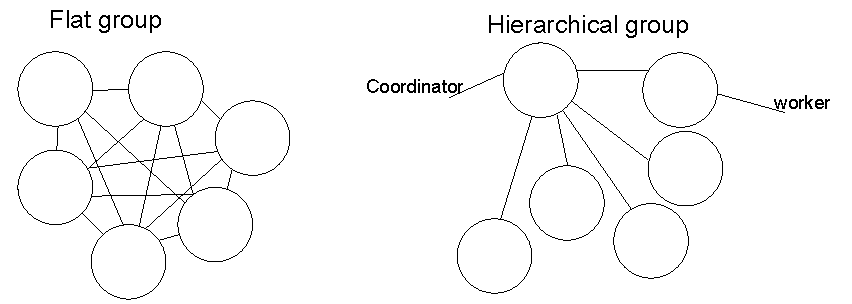
\includegraphics[width=16cm, height=7cm]{fault_masking.pdf}
\vspace{-0.5cm}\caption{Flat group and hierarchical group masking}
\label{fig:4}
%\label{fig:flate}
\end{figure}

%I would also like to add an extra bookmark in acroread like so ...
\ifpdf
  \pdfbookmark[2]{bookmark text is here}{And this is what I want bookmarked}
\fi
% ------------------------------------------------------------------------


%%% Local Variables: 
%%% mode: latex
%%% TeX-master: "../thesis"
%%% End: 

%\renewcommand{\chaptername}{HPC in the Cloud, Concepts and Architecture}
{\singlespacing{\chapter{Theory, Concepts and Architecture ...}}}
\ifpdf
    \graphicspath{{Chapter2/Chapter2Figs/PNG/}{Chapter2/Chapter2Figs/PDF/}{Chapter2/Chapter2Figs/}}
\else
    \graphicspath{{Chapter2/Chapter2Figs/EPS/}{Chapter2/Chapter2Figs/}}
\fi
\doublespacing
\section{Section title}
\label{sec:3.1}
... Place your section contents ....
\subsection{first subsection}
... and some more 

\section{Section title}
\label{sec:3.2}
... Place your section contents ....
\subsection{Second subsection }
... and some more 

\section{Section title}
\label{sec:3.3}
... Place your section contents ....

\section{Section title}
\label{sec:3.4}
... Place your section contents ....

\section{Section title}
\label{sec:3.5}
... Place your section contents ....

\section{Section title}
\par Citation - for example; A simple analysis of the Top500 [\citenum{Top500}] HPC ....


%There are three cloud services (PaaS, IaaS and HaaS) which are suitable for HPC systems in the cloud. There is a need to show which cloud service is cost effective for running computation-intensive applications in HPC in the cloud.
%And now I begin my second chapter here ...
%\section{Benefits of Cloud Computing with emphasis on HPC systems}
%\subsection{No initial A. investment capital}
%\subsection{Scalability and the need to provision demand}
%\subsection{High availability, fault-C. tolerance, and disasters}
%\subsection{Performance and Elasticity of the Cloud}
%\subsection{Mobility}
%\section{Types of Cloud Computing}
%... and some more ...
%\subsection{Public Cloud}
%\subsection{Private Cloud}
%\subsection{Community Cloud}
%\subsection{Hybrid Cloud}
%\subsection{Related Technologies}
%\subsection{Grid Computing}
%\subsection{Utility Computing}
%\subsection{Virtualization}
%\section{HPC Systems in the cloud}


%\section{Cloud Services}
%... and some more ...
%\subsection{Storage as a Service}
%\subsection{Application as a Service}
%\subsection{Platform as a Service}
%\subsection{Infrastructure as a Service}
%\subsection{Hardware as a Service}

%\section{Cost-effective Cloud Services for HPC systems}
%\subsection{Cluster Compute Instance from Amazon EC2 (IaaS)}
%\subsection{Cluster Computer Instance from HaaS}
%\section{MPI Applications and Benchmark}
%\section{Evaluation}
%\section{Cost Analysis}
%... and some more ...

%\section{Summary}
% ------------------------------------------------------------------------

%%% Local Variables: 
%%% mode: latex
%%% TeX-master: "../thesis"
%%% End: 

{\singlespacing{\chapter{Design and Implementation ... \\ }}
\ifpdf
    \graphicspath{{Chapter3/Chapter3Figs/PNG/}{Chapter3/Chapter3Figs/PDF/}{Chapter3/Chapter3Figs/}}
\else
    \graphicspath{{Chapter3/Chapter3Figs/EPS/}{Chapter3/Chapter3Figs/}}
\fi
\doublespacing

\section{Section title}
\label{sec:4.1}
... Place your section contents ....
\subsection{first subsection}
... and some more 

\section{Section title}
\label{sec:4.2}
... Place your section contents ....
\subsection{Second subsection }
... and some more 

\section{Section title}
\label{sec:4.3}
... Place your section contents ....

\section{Section title}
\label{sec:4.4}
... Place your section contents ....

Your table can also be placed here e.g., 
\begin{table}[h]
\centering
  \caption{Sample}
{\begin{tabular}{@{}lccccccc} \hline
N${_n}$	&N${_{cr}}$	&P${_{size}}$	&\$${_{ch}}$	&\$${_{r =1}}$	&\$${_{rn}}$	&\$${_{FTDaemon}}$\\[0.5ex]
 \hline

2	&2	&2000	&97.81		&74.14	&81.14	&81.14\\[1ex]

2	&3	&4000	&88.20		&68.45	&125.20	&83.47\\[1ex]

4	&5	&6000	&268.28		&214.86	&321.07	&256.85\\[1ex]

8	&10	&8000	&1266.14		&879.58	&1153.46		&1025.29\\[1ex]

16	&18	&10000	&4102.82	 	&2669.52 	&3857.88		&3429.23\\[1ex]

  \end{tabular}}
\end{table}

\section{Section title}
\label{sec:4.5}
... Place your section contents ....

{\singlespacing{\chapter{Testing and Results ... }}}
\ifpdf
    \graphicspath{{Chapter4/Chapter4Figs/PNG/}{Chapter4/Chapter4Figs/PDF/}{Chapter4/Chapter4Figs/}}
\else
    \graphicspath{{Chapter4/Chapter3Figs/EPS/}{Chapter4/Chapter3Figs/}}
\fi
\doublespacing
%\section{Introduction}
\section{Section title}
\label{sec:5.1}
... Place your section contents ....
\subsection{first subsection}
... and some more 

\section{Section title}
\label{sec:5.2}
... Place your section contents ....
\subsection{Second subsection }
... and some more 

\section{Section title}
\label{sec:5.3}
... Place your section contents ....

\section{Section title}
\label{sec:5.4}
... Place your section contents ....

\section{Section title}
\label{sec:5.5}
... Place your section contents ....

Citation e.g., Public clouds promise the major benefits of cloud computing [\citenum{armbrust2010view}] and ...



%\section{Summary}

% ------------------------------------------------------------------------


%%% Local Variables: 
%%% mode: latex
%%% TeX-master: "../thesis"
%%% End: 
%\chapter{Conclusion and Future Work}
\ifpdf
    \graphicspath{{Chapter5/Chapter5Figs/PNG/}{Chapter5/Chapter5Figs/PDF/}{Chapter5/Chapter5Figs/}}
\else
    \graphicspath{{Chapter5/Chapter5Figs/EPS/}{Chapter5/Chapter5Figs/}}
\fi

... Place your section contents ....






% ------------------------------------------------------------------------


%%% Local Variables: 
%%% mode: latex
%%% TeX-master: "../thesis"
%%% End: 

\def\baselinestretch{1}
\chapter{Conclusions and Future work}
\ifpdf
    \graphicspath{{Conclusions/ConclusionsFigs/PNG/}{Conclusions/ConclusionsFigs/PDF/}{Conclusions/ConclusionsFigs/}}
\else
    \graphicspath{{Conclusions/ConclusionsFigs/EPS/}{Conclusions/ConclusionsFigs/}}
\fi

\def\baselinestretch{1.66}

... Place your section contents ....

%%% ----------------------------------------------------------------------

% ------------------------------------------------------------------------

%%% Local Variables: 
%%% mode: latex
%%% TeX-master: "../thesis"
%%% End: 


\appendix
\chapter{}

and here I put a bit of postamble ...

% ------------------------------------------------------------------------

%%% Local Variables: 
%%% mode: latex
%%% TeX-master: "../thesis"
%%% End: 

\chapter{Appendix}

and here I put some more postamble ...

% ------------------------------------------------------------------------

%%% Local Variables: 
%%% mode: latex
%%% TeX-master: "../thesis"
%%% End: 



%\bibliographystyle{Classes/CUEDbiblio}
%\bibliographystyle{Classes/jmb}
\bibliographystyle{ieeetr} %ieeetrthis works with package natbib
%\bibliographystyle{Classes/jmb} % bibliography style
%\renewcommand{\bibname}{References} % changes default name Bibliography to References
\bibliography{References/references} % References file
\addcontentsline{toc}{chapter}{References} %adds References to contents page
%\bibliographystyle{amsplain}
%\bibliography{references}
\end{document}

